%compiling with XeLaTeX
\documentclass[twoside,11pt,abstracton]{scrreprt}

%personel data
\title{Differentialgeometrie I}
\author{Dr. Anna Siffert}
\date{Sommersemester 2018}


%math and theorems
\usepackage{amsmath}
\usepackage{amssymb}
\usepackage[amsmath,thmmarks,hyperref]{ntheorem}

%language settings and microtype
\usepackage{fontspec} 
\setmainfont{Palatino}
\setsansfont{Optima}
\setmonofont[Scale=MatchLowercase]{Menlo}

\usepackage{polyglossia}
\setmainlanguage{german}
\setotherlanguages{english}
\usepackage{microtype}

%useful packages
\usepackage{geometry}
\usepackage{xcolor}
\usepackage{graphicx}
\usepackage{float}
\usepackage{fancyhdr}
\usepackage{csquotes}
\usepackage{blindtext}
\usepackage{todonotes}


%geometry
\geometry{
	width=150mm,
	bindingoffset=7mm,}

%color settings
\definecolor{myred}{RGB}{196,19,47} 
\definecolor{myblue}{RGB}{0,139,139}


%for empty pages at the beginning of the document
\def\blankpage{%
	\clearpage%
	\thispagestyle{empty}
	\addtocounter{page}{-1}
	\null%
	\clearpage}

% Page layout for beginning of chapter
\fancypagestyle{plain}{%
	\fancyhf{}  % clear all header and footer fields 
	\fancyfoot[C]{- \thepage\hspace{3pt}-} 
	\renewcommand{\headrulewidth}{0pt}
	\renewcommand{\footrulewidth}{0pt}}

%page layout for the other pages
\pagestyle{fancy}
\fancyhf{}
\fancyhead[LE]{\textit{\nouppercase{\leftmark}}}
\fancyhead[RO]{\textit{\nouppercase{\rightmark}}}
\fancyfoot[C]{- \thepage\hspace{3pt}-}
\renewcommand{\headrulewidth}{0.2pt}
\renewcommand{\footrulewidth}{0pt}

% titles and stuff
\setkomafont{chapter}{\normalfont\bfseries\Huge}
\setkomafont{section}{\normalfont\bfseries\LARGE}
\setkomafont{subsection}{\normalfont\bfseries\large}
\setkomafont{title}{\normalfont\bfseries\Large}
\setkomafont{author}{\normalfont\bfseries\Large}
\setkomafont{date}{\normalfont\bfseries\Large}

%nice boxes
\usepackage[many]{tcolorbox}    
\newtcolorbox{mybox}[1]{%
	tikznode boxed title,
	enhanced,
	arc=0mm,
	interior style={white},
	attach boxed title to top center= {yshift=-\tcboxedtitleheight/2},
	fonttitle=\large\bfseries,
	colbacktitle=white,coltitle=black,
	boxed title style={size=normal,colframe=white,boxrule=0pt},
	title={#1}}

%proofs,defs ...

%Theorems
\theoremstyle{marginbreak}
\theoremheaderfont{\normalfont\bfseries}
\theorembodyfont{\slshape} 
\theoremseparator{}
\newtheorem{satz}{Satz}[chapter]

%Lemma
\theoremstyle{changebreak} 
\theoremindent0.5cm 
\theoremseparator{}
\newtheorem{lem}[satz]{Lemma}

%Corolarys
\theoremindent0cm 
\theoremseparator{}
\newtheorem{kor}[satz]{Korollar}

%Examples
\theoremstyle{break} 
\theorembodyfont{\upshape} 
\theoremseparator{} 
\newtheorem{bsp}[satz]{Beispiel}

%Comments; Mathieu, do your design
\theoremstyle{break} 
\theorembodyfont{\upshape} 
\theoremseparator{} 
\newtheorem*{bem}[satz]{Bemerkung}

%Definitions
\theoremstyle{break}
\theoremseparator{} 
\newtheorem{defs}[satz]{Definition}

%Proofs
%\theoremheaderfont{\normalfont} %falls es nicht dick gedruckt sein soll
\theoremstyle{nonumberbreak}
\theoremseparator{} 
\theoremsymbol{\ensuremath{\square}}
\newtheorem{bew}[satz]{Beweis:}

%bibliography
\usepackage[
style=numeric-comp,
backend=biber,
maxnames=10,
maxcitenames=2,
isbn=false,
date=year,
url=false,
doi=false
]{biblatex}
\bibliography{bibliography/diffgeo-bib}

%appendix
\usepackage[toc,page]{appendix}

%always use hyperref at the end of the preamble!
\usepackage[colorlinks=True]{hyperref}
\hypersetup{allcolors=myred}

%useful new defintions and stuff

\newcommand{\R}{\mathbb{R}}	%simplify R^n
\newcommand{\set}[1]{\{#1\}}	%siplify sets
\newcommand{\difM}{differenzierbare Mannigfaltigkeit}		%abbreveiate "differenzierbare Mannigfaltigkeit"

\begin{document}
	
%title, abstract and toc	 
\pagenumbering{roman} %start roman numbering before main text

\begin{titlepage}
	\begin{center}
		\makeatletter
		
		\thispagestyle{empty}
		
		\Huge\textbf{\@title} \\
		\vspace{5mm}
		\Large\textbf{ gehalten von \@author} \\
		\large{im \@date} \\
		\vspace{5mm}
		\large{an der} \\
		\Large\textbf{Ruprecht-Karls-Universität Heidelberg} \\
		\vfill
		\begin{figure}[H]
			\centering
			\includegraphics*[width=0.6\textwidth]{figures/logo-uni-hd-small}
		\end{figure}
	    \vfill
		\Large
		In \LaTeX \ gesetzt von \\ 
		\vspace{3mm}
		\bfseries{
		Mathieu Kaltschmidt
		\& 
		Quirinus Schwarzenböck}\\ 	
	   \vfill
	   \normalfont
	   aktueller Stand: \  \textit{\today}
	   \vfill
		\makeatother
	\end{center}
\blankpage
\end{titlepage}

{\renewcommand{\headrulewidth}{0pt} % kill headrule for abstract and toc
	\addcontentsline{toc}{chapter}{Vorwort}
	\makeatletter

\begin{figure}[H]
\flushright

\includegraphics[width=0.4\textwidth]{figures/logo-uni-hd}
\end{figure}
\vspace{-30mm}
\begin{flushleft}	
\textbf{\LARGE\@title} \\
\vspace{0.5cm}
\Large\@author \\
\end{flushleft}
\vspace{5mm}
\rule{\textwidth}{0.2pt}

\makeatother

\vfill

{\let\raggedsection\centering
\section*{Vorwort}
\blindtext

% books and more
\printbibliography[heading=none]


\blindtext

\vfill

\blankpage
	\tableofcontents
	\blankpage}
}
%main content
\setcounter{tocdepth}{1}
\pagenumbering{arabic} % now set main numbering in arabic

%lectures
\chapter{Differenzierbare Mannigfaltigkeiten}
\section*{Worum geht es in der Differentialgeometrie?}
Die zentralen Objekte der Differentialgeometrie sind Mannigfaltigkeiten. Das Ziel ist es, Analysis und Geometrie auf solchen Mannigfaltigkeiten zu betreiben. \\
Wir beginnen zunächst einmal mit einer kurzen Gegenüberstellung der bereits bekannten Konzepte aus dem $\mathbb{R}^n$ mit den korrespondierenden Begriffen der Differentialgeometrie, welche wir in den kommenden Vorlesungen noch genauer kennenlernen werden.

%Vergleich
\begin{figure}[H]
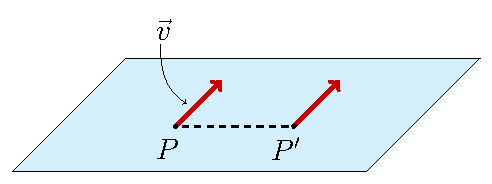
\includegraphics[scale=0.8]{figures/tikz/plane.pdf}
\hspace{2cm}
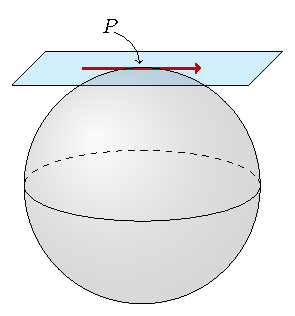
\includegraphics[scale=0.9]{figures/tikz/sphere_with_plane.pdf}
\end{figure}

\begin{figure}[H]
\centering
\begin{tabular}{>{\centering}p{.45\textwidth} | >{\centering}p{.45\textwidth}} 
$\mathbb{R}^n$ \vspace{5pt} & $\Huge\mathcal{M}$  \vspace{5pt} \tabularnewline \hline 
\vspace{5pt} Parallelverschiebung & \vspace{5pt} Begriff des Zusammenhangs\tabularnewline 
\vspace{5pt} Gerade = kürzeste Verbindung & \vspace{5pt} Konzept der Geodätischen \tabularnewline 
\vspace{5pt} flacher Raum & \vspace{5pt} gekrümmter Raum \tabularnewline 
\vspace{5pt} Skalarprodukt & \vspace{5pt} Riemannsche Metrik \tabularnewline 
\end{tabular}
\end{figure}
\section{Definitionen}
Um differenzierbare Mannigfaltigkeiten definieren zu können wiederholen wir zunächst die Definition eines topologischen Raumes. \\
\phantom{.}\\
\bfseries Erinnerung: \normalfont $M \subseteq \mathbb{R}^n$ offen, wenn $\forall p \in U \ \exists \ \varepsilon>0$, sodass $B_{\varepsilon}(p) \subset U$. Dieser Begriff von Offenheit heißt \textit{euklidische Topologie} \normalfont und erfüllt:
\begin{enumerate}
\item[i)] $\emptyset, \mathbb{R}^n$ offen
\item[ii)] $U, V \subset \mathbb{R}^n$ offen $\Rightarrow U \cap V$ offen in $\mathbb{R}^n$
\item [iii)] $U_i, i \in $ I offen in $\mathbb{R}^n \Rightarrow \bigcup\limits_{i \in \text{I}} U_i \subset \mathbb{R}^n$ offen
\end{enumerate} 
\begin{defs}[Topologischer Raum]
Ein topologischer Raum ist eine Menge $X$ zusammen mit einer Menge $\mathcal{O} \subset \mathcal{P}(X)$, sodass:
\begin{enumerate}
	\item[i)] $\emptyset, X \in \mathcal{O}$
	\item[ii)] $U, V \in \mathcal{O} \Rightarrow  U \cap V \in \mathcal{O}$
	\item [iii)] $U_i \in \mathcal{O} \Rightarrow\bigcup\limits_{i \in \text{I}} U_i \in \mathcal{O}$
\end{enumerate} 
\end{defs}
\begin{bsp}
\begin{enumerate}
	\item[a)] $( X, \mathcal{O} = \mathcal{P}(x) )$
	\item[b)] $N \subset X$ Teilmenge. Dann ist auch $(N,\mathcal{O}_1)$ ein topologischer Raum, wobei $\mathcal{O}_1$ wie folgt gegeben ist:\\
	\center{$V \in \mathcal{O}_1 \Leftrightarrow \ \exists \ U \in \mathcal{O}$, sodass $V= N \cap U$}
\end{enumerate}
Teilmengen topologischer Räume sind topologische Räume.
\end{bsp}

\begin{defs}[Topologische Mannigfaltigkeiten]
Eine topologische Mannigfaltigkeit ist ein topologischer Raum $\mathcal{M}$ der Dimension $n$ mit folgenden Eigenschaften:
\begin{enumerate}
	\item[i)] $\mathcal{M}$ ist hausdorffsch. Das heißt $\forall \ p, q \in \mathcal{M}$ mit $p \neq q \  \exists$ \ zwei disjunkte, offene Umgebungen $U \in p$ und $V \in q$ wobei $U, V \in \mathcal{O}$
	\item[ii)] \textbf{2. Abzählbarkeitsaxiom}  \\
	$\mathcal{M}$ hat eine abzählbare Basis der Topologie, das heißt es existieren abzählbar viele Mengen $\{U_1, \dots, U_k, \dots\}$ offener Teilmengen mit $U_i \in \mathcal{O}$, sodass $\forall p \in \mathcal{M}$ und alle Umgebungen $U$ von $p$ gibt es ein $K$ sodass $p \in U_k \subseteq U$.
	\item [iii)] $\mathcal{M}$ ist homöomorph zu $\mathbb{R}^n$, das heißt $\forall p \in \mathcal{M}$ existiert eine Umgebung $U$ von $p$ und ein \bfseries Homöomorphismus \normalfont $X: U \rightarrow V \subseteq \mathbb{R}^n$ (offen).
\end{enumerate} 
\end{defs}

\begin{defs}[Karte, Atlas]
Das Paar $(X, U)$ heißt \textbf{Karte} von $\mathcal{M}$ um $p$. \\
Eine Menge $\mathcal{A} = \{(x_{\alpha},U_{\alpha})_{\alpha \in \mathcal{A}}\}$ von Karten hießt \textbf{Atlas} von $\mathcal{M}$, falls \\
\begin{align}
\bigcup\limits_{\alpha \in \mathcal{A}} = \mathcal{M}
\end{align}
\end{defs}

Topologische Mannigfaltigkeiten sind die Grundbausteine. Nun wollen wir auf diesen Mannigfaltigkeiten Geometrie betreiben. Dafür benötigen wir mehr Struktur. Wir wollen die differenzierbare Struktur des $\mathbb{R}^n$ auf unseren Mannigfaltigkeiten "holen".

\begin{defs}[Kartenwechsel]
Seien $x_{\alpha}$ und $x_{\beta}$ zwei Karten, dann ist der Kartenwechsel wie folgt definiert: \\
\begin{align}
x_{\alpha}\circ x_{\beta}^{-1}: x_{\beta}(U_{\alpha}\cap U_{\beta}) \rightarrow x_{\alpha}(U_{\alpha}\cap U_{\beta}) \subseteq \mathbb{R}^n
\end{align}
Dies ist ein Homöomorphismus.
\end{defs}
Nun wollen wir, dass $x_{\alpha}\circ x_{\beta}^{-1}$ Diffeomorphismen sind.

\begin{defs}
Sei $ \mathcal{M}$ eine topologische Mannigfaltigkeit.
\begin{enumerate}
	\item[a)] Ein Atlas $\mathcal{A} = \{(x_{\alpha},U_{\alpha})\}$ auf $\mathcal{M}$ heißt $C^{\infty}$-Atlas, falls alle Kartenwechsel $x_{\alpha}\circ x_{\beta}^{-1}$ mit $\alpha, \beta \in A \ C^{\infty}$-Diffeomorphismen sind.
	\item[b)] Sei $\mathcal{A}$ ein $C^{\infty}$-Atlas von $\mathcal{M}$. \\
	Eine Karte $(x,U)$ ist verträglich mit $\mathcal{A}$, falls $x \circ x^{-1}$ ein $C^{\infty}$-Diffeomorphismus ist.
\end{enumerate}
\end{defs}
Gegeben ein $C^{\infty}$-Atlas, so kann man diesen zu einem \textit{maximalen} $C^{\infty}$-Atlas vervollständigen. Maximal bedeutet hierbei, dass der Atlas nicht strikt in einem anderen enthalten ist.


\begin{defs}[Differenzierbare Mannigfaltigkeit]
Eine \textit{differenzierbare Struktur} auf einer topologischen Mannigfaltigkeit M ist ein \textit{maximaler $C^\infty$-Atlas}. Eine \textit{differenzierbare Mannigfaltigkeit} ist eine topologische Mannigfaltigkeit mit einer differenzierbaren Struktur.
\end{defs}

\begin{bem}
Man kann auch eine topologische Mannigfaltigkeit definieren, ohne das 2. Abzählbarkeitsaxiom zu fordern.
\begin{description}
\item[Aber:] Dann bekommt man Mannigfaltigen mit ganz anderen Eigenschaften als diejenigen, die wir betrachten wollen.
\item[Wichtig:] Hausdorffsch + 2. Abzählbarkeitsaxiom $\Rightarrow$ parakompakt, d. h. jede offene Überdeckung hat eine lokale Verfeinerung.
\end{description}
$(V_j)$ heißt Verfeinerung von $(U_j)$, falls $\forall V_j \exists U_j$ mit $V_j \subseteq U_j$\\
Lokal endlich: $\forall p \in X\ \exists$ Umgebung $U$, die nur endlich viele $U_i$ trifft\\
Parakompakt $\Rightarrow \exists$ Partition der Eins f mit 
\begin{align*}
f_i: V_i \subseteq X \rightarrow [0, 1],\ \sum_{i \in I} f_i (x) = 1
\end{align*} 
\end{bem}

\begin{bsp}
Metrische Räume sind parakompakt.
\end{bsp}

\begin{bsp}[differenzierbare Mannigfaltigkeiten]
\begin{enumerate}
\item$\mathbb{R}^n$ mit Atlas $\mathcal{A} = \{(\operatorname{id}, \R^n)\}$
\item$V$ Vektorraum, $B$ Basis mit $B = \{v_1, \cdots, v_n\}$, Atlas $\mathcal{A} = \set{(\chi_B, V)}$
\begin{align*}
& \chi_B: V \rightarrow \R^n\\
& v = \sum^n_{i=1} a_i v_i \mapsto \sum_{i=1}^n a_i e_i
\end{align*}
wobei $(e_1, \cdots, e_n)$ die Standartbasis ist.
\item$M\subseteq \R^n,\ (\chi_U, U)$ mit $\chi_U = \operatorname{id}\vert_U,\ V \subseteq M^n,\ M$ differenzierbare Mannigfaltigkeit, $\mathcal{A} = \set{(\chi_X, U)}$ Atlas von $M$\\
$\mathcal{A}_V = \set{(\chi_V, U_V}$ wobei $(\chi_V, U_V) = (\chi_{U\cap V}, U\cap V)$
\item$M_1 = S^1,\ M_2 = \R,\ M_1\times M_2 =$ "unendlicher Zylinder"
\end{enumerate}
\hspace{.06\textwidth}
\begin{minipage}[H]{0.8\textwidth}
Seien $M_1^{n_1}, M_1^{n_2}$ differenzierbare Mannigfaltigkeiten, so ist $M_1\times M_2$ ebenfalls eine \difM \ der Dimension $n_1 + n_2$.\\
Atlas $\mathcal{A} = \set{(x\times y, U\times V)}$, wobei 
\begin{align*}
(x, U) &= \text{Karte von } M_1\\
(y, V) &= \text{Karte von } M_2
\end{align*}
$(x\times y)(p_1, p_2) = (x(p_1), y(p_2))$
\end{minipage}
\hspace{1cm}
\begin{minipage}[H]{.2\textwidth}
\vspace{-1.5cm}

\includegraphics[scale=0.5]{figures/tikz/cylinder.pdf}
\end{minipage}
\end{bsp}

\begin{bem}
$N$ mit der Teilraumtopologie und dem Atlas $\mathcal{A}_N = \set{(\chi\vert_U, U\cap N)}$ ist eine \difM.
\end{bem}

\begin{defs}
Seien $M, N$ differenzierbare Mannigfaltigkeiten. Eine \textit{Einbettung} ist eine differenzierbare Abbildung
\begin{align*}
f: N \rightarrow M
\end{align*}
sodass
\begin{enumerate}
\item$f(N)\subset M$ eine Untermannigfaltigkeit 
\item$f: N \rightarrow f(N)$ Diffeomorphismus
\end{enumerate}
\end{defs}

\section{Tangentialraum} 

\missingfigure{Tangentialräume}

\begin{defs}
\begin{enumerate}
\item Ein Tangentialvektor an $M$ im Punkt $p \in M$ ist eine $\R$-lineare Abbildung
\begin{align*}
v: \mathcal{F}(M) \rightarrow \R
\end{align*}
mit $v(fg) = v(f)g(p) + f(p)v(g)$.
\item Die Menge aller Tangentialvektoren an $M$ in $p$ heißt \textit{Tangentialraum} von $M$ in $p$: $T_pM$\\
$T_pM$ ist ein Vektorraum.
\end{enumerate}
\end{defs}

\begin{hlem}[Existenz einer Glockenfunktion]
Sei $U \subseteq M$ offen, $p \in U$. Dann $\exists \varphi \in \mathcal{F}(M)$, s. d. 
\begin{enumerate}
\item$\operatorname{supp}\varphi\subseteq U$
\item$\varphi$ auf einer Umgebung $U' \subset U$ von $p$ ist
\end{enumerate}
\end{hlem}

\begin{bew}
Sei $(x, U)$ eine Karte um $\varphi$, $\varepsilon > 0$, s. d. $B_{2\varepsilon}(x(p))\subset V\subset \R^n$ und wähle $\psi:\R^n\rightarrow\R$ mit 
\begin{align*}
\left.
\begin{array}{r}
\operatorname{supp}(\varphi)\subset B_{2\varepsilon}(x(p))\\
\varphi = 1 \text{ auf } B_\varepsilon
\end{array}
\right\} \text{ Resultat aus Analysis}\\
\end{align*}

Setze $\varphi(q) = \left\{
\begin{array}{l}
\psi(x(q))\text{ für }q\in U\\
0 \text{ sonst}
\end{array}
\right.$
\end{bew}

\begin{satz}[Eigenschaften des Tangentialraums]
Für $v\in T_p M$ gilt:
\begin{enumerate}
\item$v(\text{konstante Funktion}) = 0$
\item Falls $f = g$ in einer Umgebung von $p$, so gilt $v(f) = v(g)$
\end{enumerate}
"Lokalisierung von Tangentialvektoren"
\end{satz}

\begin{bew}[zu 2]
Wähle $\varphi$ wie im Hilfslemma, wobei $U$so gewählt ist, dass $\varphi f = \varphi g$ auf $U$ ist. Nun gilt:
\begin{align*}
v(\varphi f) &= v(\varphi)f(p) + \varphi(p)v(f)\\
&= v(\varphi)f(p) + v(f)\\
v(\varphi g) &= v(\varphi)g(p) + v(g)
\end{align*}
Dann folgt $v(\varphi f) = v(\varphi g) \Leftrightarrow v(f) = v(g)$.
\end{bew}

\begin{bew}[zu 1]
	$v(\lambda f) = \lambda v(f),\ \lambda \in \R,\ f\in \mathcal{F}(\R)$\\
	\textit{zz:} $v(\lambda) = 0$. Aufgrund von $v(\lambda) = \lambda v(1)$ genügt es zu zeigen, dess $v(1) = 0$. Dies folgt aus der Produktregel
	\begin{align*}
	v(1) = v(1*1) = 1v(1) + v(1)1 = 2v(1) \Rightarrow v(1) = 0
	\end{align*}
\end{bew}


\include{content/VL4-260418}




%\appendix
\blankpage
\pagenumbering{Roman} %start capital roman numbering for appendices
\pagestyle{plain}
\addcontentsline{toc}{chapter}{Abbildungsverzeichnis}	
\listoffigures




\end{document}